%%%%%%%%%%%%%%%%%%%%%%%%%%%%%%%%%%%%%%%%%%%%%%%%%%%%%%%%%%%%%%%
% Smart Water Saver Agent - Project Report (LaTeX)
% Phase 3: AI Agent & Analytics
% Software Project Management (SPM)
%%%%%%%%%%%%%%%%%%%%%%%%%%%%%%%%%%%%%%%%%%%%%%%%%%%%%%%%%%%%%%%

\documentclass[12pt,a4paper]{article}

% Packages
\usepackage[utf8]{inputenc}
\usepackage[margin=1in]{geometry}
\usepackage{graphicx}
\usepackage{hyperref}
\usepackage{listings}
\usepackage{xcolor}
\usepackage{titlesec}
\usepackage{fancyhdr}
\usepackage{tikz}
\usepackage{array}
\usepackage{longtable}
\usepackage{booktabs}
\usepackage{enumitem}
\usepackage{caption}
\usepackage{subcaption}

% TikZ libraries
\usetikzlibrary{shapes.geometric, arrows, positioning, calc}

% Hyperref setup
\hypersetup{
    colorlinks=true,
    linkcolor=blue,
    filecolor=magenta,      
    urlcolor=cyan,
    pdftitle={Smart Water Saver Agent - Project Report},
    pdfauthor={SPM Team},
}

% Code listing style
\lstdefinestyle{pythoncode}{
    language=Python,
    basicstyle=\ttfamily\small,
    keywordstyle=\color{blue},
    stringstyle=\color{red},
    commentstyle=\color{gray},
    breaklines=true,
    frame=single,
    numbers=left,
    numberstyle=\tiny\color{gray},
    showstringspaces=false,
    tabsize=4
}

\lstdefinestyle{jsoncode}{
    basicstyle=\ttfamily\small,
    stringstyle=\color{red},
    breaklines=true,
    frame=single,
    showstringspaces=false,
    tabsize=2
}

% Header and footer
\pagestyle{fancy}
\fancyhf{}
\rhead{Smart Water Saver Agent}
\lhead{SPM - Phase 3}
\rfoot{Page \thepage}

% Title formatting
\titleformat{\section}{\Large\bfseries}{\thesection}{1em}{}
\titleformat{\subsection}{\large\bfseries}{\thesubsection}{1em}{}

% Document Information
\title{
    \textbf{Smart Water Saver Agent} \\
    \large Phase 3: AI Agent \& Analytics \\
    \large Project Report
}
\author{
    Software Project Management (SPM) \\
    Semester 7
}
\date{\today}

%%%%%%%%%%%%%%%%%%%%%%%%%%%%%%%%%%%%%%%%%%%%%%%%%%%%%%%%%%%%%%%
% DOCUMENT BEGIN
%%%%%%%%%%%%%%%%%%%%%%%%%%%%%%%%%%%%%%%%%%%%%%%%%%%%%%%%%%%%%%%

\begin{document}

% Title Page
\maketitle
\thispagestyle{empty}

\vspace{2cm}

\begin{center}
\large
\textbf{Domain:} Smart Water Conservation \\[0.5cm]
\textbf{Technology Stack:} Python, FastAPI, LangGraph \\[0.5cm]
\textbf{Architecture:} Supervisor-Worker (Worker Agent) \\[2cm]
\end{center}

\begin{abstract}
This report presents the design, implementation, and evaluation of the Smart Water Saver Agent, an intelligent Worker agent developed for the SPM Supervisor-Worker architecture. The agent leverages LangGraph for conversational AI and provides three core capabilities: weather-based watering recommendations, water usage analytics from long-term memory, and personalized conservation tips. The system adheres to a strict API contract, ensuring seamless integration with the Supervisor component.
\end{abstract}

\newpage
\tableofcontents
\newpage

%%%%%%%%%%%%%%%%%%%%%%%%%%%%%%%%%%%%%%%%%%%%%%%%%%%%%%%%%%%%%%%
% SECTION 1: INTRODUCTION
%%%%%%%%%%%%%%%%%%%%%%%%%%%%%%%%%%%%%%%%%%%%%%%%%%%%%%%%%%%%%%%

\section{Introduction}

\subsection{Project Overview}

The Smart Water Saver Agent is a sophisticated AI-powered Worker agent designed to promote water conservation through intelligent recommendations and analytics. Built using Python's FastAPI framework and LangChain's LangGraph library, the agent processes natural language requests and provides personalized responses based on weather forecasts and historical usage data.

\subsection{Objectives}

The primary objectives of this project are:

\begin{enumerate}
    \item \textbf{Deliverable 1 (Report):} Provide comprehensive documentation including Work Breakdown Structure (WBS), system architecture, memory management strategy, and API contract specification.
    
    \item \textbf{Deliverable 2 (Code):} Implement a robust FastAPI application that:
    \begin{itemize}
        \item Strictly adheres to \texttt{AgentRequest} and \texttt{AgentResponse} Pydantic models
        \item Implements \texttt{/health} and \texttt{/chat} endpoints
        \item Integrates LangGraph for intent-based routing
        \item Connects to external services (Weather API, Database)
    \end{itemize}
    
    \item \textbf{Deliverable 3 (Demo):} Demonstrate all agent capabilities including watering advice, usage analytics, and conservation tips.
\end{enumerate}

\subsection{Technology Stack}

\begin{table}[h]
\centering
\begin{tabular}{ll}
\toprule
\textbf{Component} & \textbf{Technology} \\
\midrule
Web Framework & FastAPI 0.104.1 \\
AI Engine & LangGraph 0.0.69 \\
LLM Integration & LangChain + OpenAI \\
Data Validation & Pydantic 2.5.0 \\
Web Server & Uvicorn 0.24.0 \\
Database & PostgreSQL (Phase 2) \\
Weather API & WeatherAPI.com \\
Testing & pytest 7.4.3 \\
Containerization & Docker \\
\bottomrule
\end{tabular}
\caption{Technology Stack}
\label{tab:tech_stack}
\end{table}

%%%%%%%%%%%%%%%%%%%%%%%%%%%%%%%%%%%%%%%%%%%%%%%%%%%%%%%%%%%%%%%
% SECTION 2: PROJECT MANAGEMENT
%%%%%%%%%%%%%%%%%%%%%%%%%%%%%%%%%%%%%%%%%%%%%%%%%%%%%%%%%%%%%%%

\section{Project Management}

\subsection{Work Breakdown Structure (WBS)}

The project was structured into six major work packages, as illustrated in Figure~\ref{fig:wbs}.

\begin{figure}[h]
\centering
\small
\begin{verbatim}
3.0 AI Agent & Analytics
├── 3.1 Project Setup & Scaffolding
│   ├── 3.1.1 Initialize Python project
│   ├── 3.1.2 Install dependencies (FastAPI, LangGraph)
│   ├── 3.1.3 Create main.py with FastAPI app
│   └── 3.1.4 Implement Pydantic models
│
├── 3.2 API Endpoint Implementation
│   ├── 3.2.1 Create /health endpoint (GET)
│   ├── 3.2.2 Create /chat endpoint (POST)
│   └── 3.2.3 Basic unit tests
│
├── 3.3 LangGraph Architecture Design
│   ├── 3.3.1 Define AgentState (TypedDict)
│   ├── 3.3.2 Create Router node
│   └── 3.3.3 Define conditional edges
│
├── 3.4 Tool & Node Implementation
│   ├── 3.4.1 Create weather tool
│   ├── 3.4.2 Create usage tool (database)
│   ├── 3.4.3 Create response generator
│   └── 3.4.4 Create fallback node
│
├── 3.5 Graph Assembly & Integration
│   ├── 3.5.1 Add nodes and edges
│   ├── 3.5.2 Compile the graph
│   └── 3.5.3 Integrate with /chat endpoint
│
└── 3.6 Testing & Documentation
    ├── 3.6.1 Write integration tests
    ├── 3.6.2 API contract documentation
    └── 3.6.3 README and deployment guides
\end{verbatim}
\caption{Work Breakdown Structure for Phase 3}
\label{fig:wbs}
\end{figure}

\subsection{Project Schedule}

Table~\ref{tab:schedule} presents the high-level schedule for the 3-week development phase.

\begin{table}[h]
\centering
\begin{tabular}{p{5cm}ccc}
\toprule
\textbf{Task} & \textbf{Week 1} & \textbf{Week 2} & \textbf{Week 3} \\
\midrule
Setup \& Scaffolding & \textcolor{blue}{████} & & \\
API Endpoint Implementation & \textcolor{blue}{████} & & \\
LangGraph Architecture & \textcolor{blue}{████} & & \\
Tool \& Node Implementation & & \textcolor{blue}{█████} & \\
Graph Assembly & & \textcolor{blue}{███} & \\
Testing \& Documentation & & & \textcolor{blue}{█████} \\
\bottomrule
\end{tabular}
\caption{Project Schedule (Gantt Chart)}
\label{tab:schedule}
\end{table}

\subsection{Risk Management}

Table~\ref{tab:risks} outlines identified risks and mitigation strategies.

\begin{table}[h]
\centering
\small
\begin{tabular}{p{1cm}p{4cm}p{1.5cm}p{1.5cm}p{5cm}}
\toprule
\textbf{ID} & \textbf{Risk} & \textbf{Probability} & \textbf{Impact} & \textbf{Mitigation} \\
\midrule
R-01 & Intent misclassification & Medium & High & Robust fallback node with clarification prompts \\
\midrule
R-02 & External API failure & Medium & Medium & Timeouts, caching, circuit breakers, mock fallback \\
\midrule
R-03 & API contract mismatch & Low & High & Strict Pydantic validation, schema tests \\
\midrule
R-04 & Database latency & Medium & Medium & Pagination, 7-day default query limit \\
\bottomrule
\end{tabular}
\caption{Risk Assessment and Mitigation}
\label{tab:risks}
\end{table}

%%%%%%%%%%%%%%%%%%%%%%%%%%%%%%%%%%%%%%%%%%%%%%%%%%%%%%%%%%%%%%%
% SECTION 3: SYSTEM ARCHITECTURE
%%%%%%%%%%%%%%%%%%%%%%%%%%%%%%%%%%%%%%%%%%%%%%%%%%%%%%%%%%%%%%%

\section{System Architecture}

\subsection{High-Level Architecture}

Figure~\ref{fig:architecture} illustrates the overall system architecture showing the interaction between the Supervisor, the Worker agent, and external services.

\begin{figure}[h]
\centering
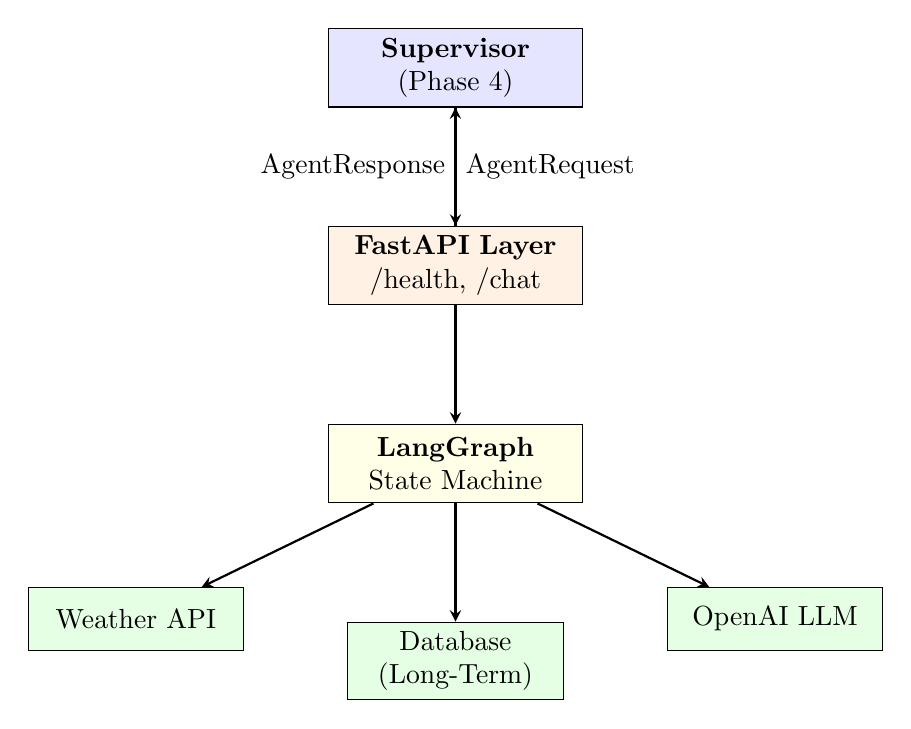
\begin{tikzpicture}[
    node distance=1.5cm,
    box/.style={rectangle, draw, fill=blue!10, text width=3cm, text centered, minimum height=1cm},
    tool/.style={rectangle, draw, fill=green!10, text width=2.5cm, text centered, minimum height=0.8cm},
    arrow/.style={thick,->,>=stealth}
]

% Supervisor
\node[box] (supervisor) at (0,0) {\textbf{Supervisor} \\ (Phase 4)};

% Agent Layer
\node[box, below=of supervisor, fill=orange!10] (fastapi) {\textbf{FastAPI Layer} \\ /health, /chat};
\node[box, below=of fastapi, fill=yellow!10] (langgraph) {\textbf{LangGraph} \\ State Machine};

% Tools
\node[tool, below left=of langgraph] (weather) {Weather API};
\node[tool, below=of langgraph] (database) {Database \\ (Long-Term)};
\node[tool, below right=of langgraph] (llm) {OpenAI LLM};

% Arrows
\draw[arrow] (supervisor) -- node[right] {AgentRequest} (fastapi);
\draw[arrow] (fastapi) -- (langgraph);
\draw[arrow] (langgraph) -- (weather);
\draw[arrow] (langgraph) -- (database);
\draw[arrow] (langgraph) -- (llm);
\draw[arrow] (fastapi) -- node[left] {AgentResponse} (supervisor);

\end{tikzpicture}
\caption{High-Level System Architecture}
\label{fig:architecture}
\end{figure}

\subsection{LangGraph State Machine}

The core of the agent is a LangGraph state machine that routes user requests based on classified intent. Figure~\ref{fig:langgraph} shows the state transition diagram.

\begin{figure}[h]
\centering
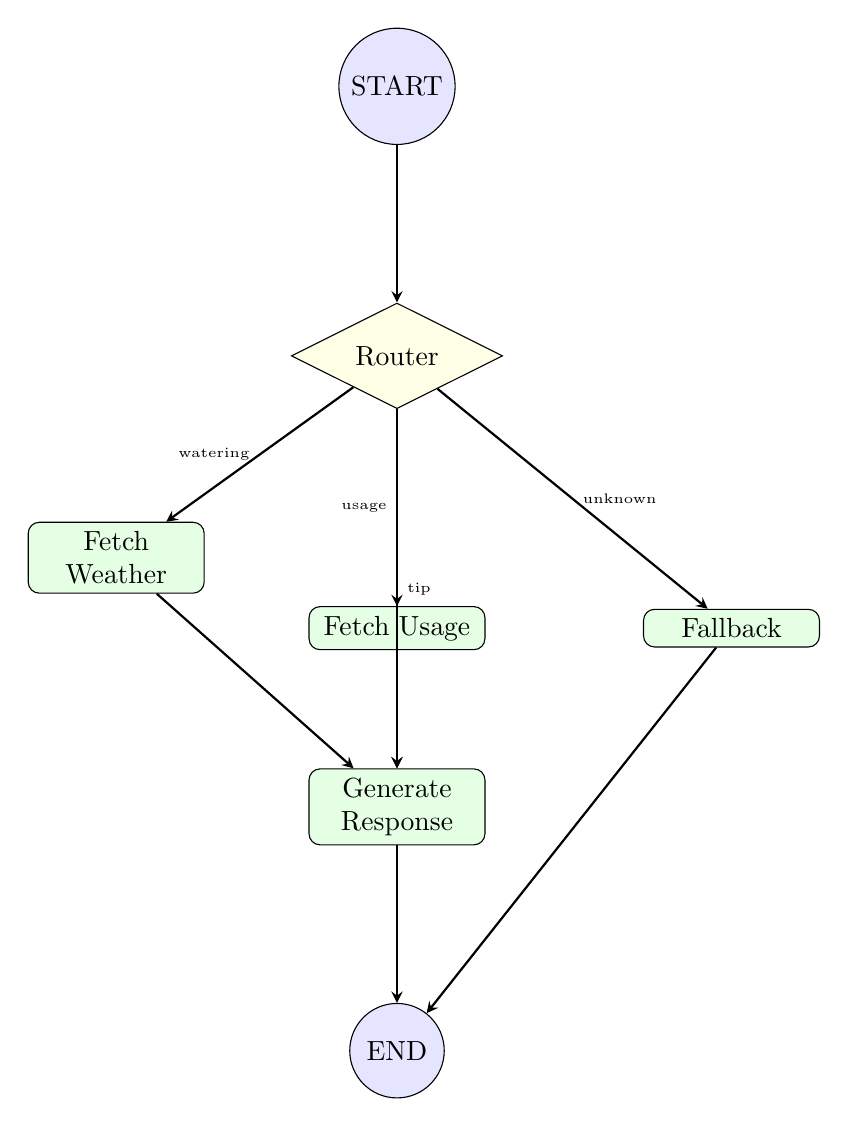
\begin{tikzpicture}[
    node distance=2cm,
    state/.style={circle, draw, fill=blue!10, minimum size=1.2cm},
    decision/.style={diamond, draw, fill=yellow!10, aspect=2, text width=1.5cm, text centered},
    tool/.style={rectangle, rounded corners, draw, fill=green!10, text width=2cm, text centered},
    arrow/.style={thick,->,>=stealth}
]

% Nodes
\node[state] (start) {START};
\node[decision, below=of start] (router) {Router};
\node[tool, below left=2.5cm of router] (weather) {Fetch Weather};
\node[tool, below=2.5cm of router] (usage) {Fetch Usage};
\node[tool, right=of usage] (fallback) {Fallback};
\node[tool, below=1.5cm of usage] (generate) {Generate Response};
\node[state, below=of generate] (end) {END};

% Arrows
\draw[arrow] (start) -- (router);
\draw[arrow] (router) -- node[left, font=\tiny] {watering} (weather);
\draw[arrow] (router) -- node[left, font=\tiny] {usage} (usage);
\draw[arrow] (router) -- node[right, font=\tiny] {tip} (generate);
\draw[arrow] (router) -- node[right, font=\tiny] {unknown} (fallback);
\draw[arrow] (weather) -- (generate);
\draw[arrow] (usage) -- (generate);
\draw[arrow] (fallback) -- (end);
\draw[arrow] (generate) -- (end);

\end{tikzpicture}
\caption{LangGraph State Machine Flow}
\label{fig:langgraph}
\end{figure}

\subsection{AgentState Definition}

The state object passed between nodes is defined as:

\begin{lstlisting}[style=pythoncode]
class AgentState(TypedDict):
    messages: Annotated[Sequence[BaseMessage], operator.add]
    user_id: Optional[str]
    intent: Optional[str]
    weather_data: Optional[dict]
    usage_data: Optional[dict]
    final_response: Optional[str]
\end{lstlisting}

%%%%%%%%%%%%%%%%%%%%%%%%%%%%%%%%%%%%%%%%%%%%%%%%%%%%%%%%%%%%%%%
% SECTION 4: MEMORY STRATEGY
%%%%%%%%%%%%%%%%%%%%%%%%%%%%%%%%%%%%%%%%%%%%%%%%%%%%%%%%%%%%%%%

\section{Memory Strategy}

\subsection{Short-Term Memory (Ephemeral)}

\textbf{Implementation:} LangGraph State (\texttt{messages} field)

\textbf{Purpose:} Maintains conversational context within a single request

\textbf{Lifecycle:} Created at request initialization, destroyed after response

\textbf{Benefits:}
\begin{itemize}
    \item Enables multi-turn conversations
    \item Provides context for coherent responses
    \item Zero persistence overhead
\end{itemize}

\subsection{Long-Term Memory (Persistent)}

\textbf{Implementation:} Phase 2 Database (PostgreSQL)

\textbf{Purpose:} Historical water usage data for analytics and personalization

\textbf{Access Pattern:} Via \texttt{fetch\_usage} tool node

\textbf{Data Retrieved:}
\begin{itemize}
    \item User consumption history (configurable period, default: 7 days)
    \item Usage patterns and trends
    \item Peak usage analytics
    \item Device-specific consumption data
\end{itemize}

\textbf{Benefits:}
\begin{itemize}
    \item Single source of truth (no data duplication)
    \item Scalable to all users
    \item Enables personalized recommendations
    \item Supports pattern analysis and predictions
\end{itemize}

\subsection{Memory Flow Example}

Figure~\ref{fig:memory_flow} illustrates how the agent combines both memory types.

\begin{figure}[h]
\centering
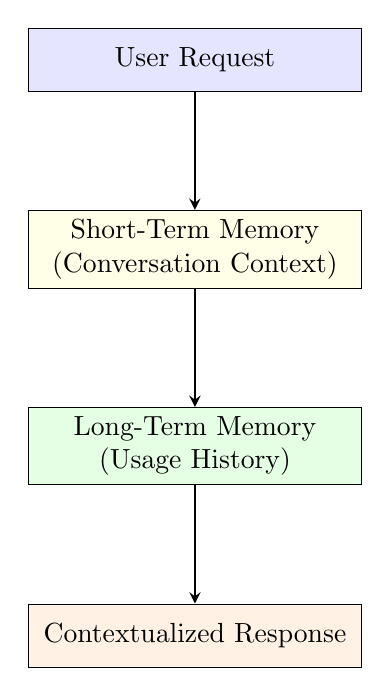
\begin{tikzpicture}[
    node distance=1.5cm,
    box/.style={rectangle, draw, text width=4cm, text centered, minimum height=0.8cm},
    arrow/.style={thick,->,>=stealth}
]

\node[box, fill=blue!10] (request) {User Request};
\node[box, fill=yellow!10, below=of request] (shortterm) {Short-Term Memory \\ (Conversation Context)};
\node[box, fill=green!10, below=of shortterm] (longterm) {Long-Term Memory \\ (Usage History)};
\node[box, fill=orange!10, below=of longterm] (response) {Contextualized Response};

\draw[arrow] (request) -- (shortterm);
\draw[arrow] (shortterm) -- (longterm);
\draw[arrow] (longterm) -- (response);

\end{tikzpicture}
\caption{Memory Integration Flow}
\label{fig:memory_flow}
\end{figure}

%%%%%%%%%%%%%%%%%%%%%%%%%%%%%%%%%%%%%%%%%%%%%%%%%%%%%%%%%%%%%%%
% SECTION 5: API CONTRACT
%%%%%%%%%%%%%%%%%%%%%%%%%%%%%%%%%%%%%%%%%%%%%%%%%%%%%%%%%%%%%%%

\section{API Contract}

\subsection{Overview}

All endpoints conform to standardized Pydantic models ensuring type safety and consistency with the Supervisor interface.

\subsection{Health Check Endpoint}

\textbf{Endpoint:} \texttt{GET /health}

\textbf{Description:} Provides operational status for monitoring

\textbf{Response Schema:}
\begin{lstlisting}[style=jsoncode]
{
  "agent_name": "SmartWaterSaverAgent",
  "status": "success",
  "data": {
    "message": "Agent is operational",
    "version": "1.0.0",
    "capabilities": [
      "watering_advice",
      "usage_query",
      "general_tip"
    ]
  },
  "error_message": null
}
\end{lstlisting}

\subsection{Chat Endpoint}

\textbf{Endpoint:} \texttt{POST /chat}

\textbf{Description:} Main conversational interface

\textbf{Request Schema (\texttt{AgentRequest}):}
\begin{lstlisting}[style=jsoncode]
{
  "messages": [
    {
      "role": "user",
      "content": "Should I water my garden today?"
    }
  ],
  "user_id": "optional_string"
}
\end{lstlisting}

\textbf{Success Response (\texttt{AgentResponse}):}
\begin{lstlisting}[style=jsoncode]
{
  "agent_name": "SmartWaterSaverAgent",
  "status": "success",
  "data": {
    "content": "No, I would not recommend watering 
               today. The forecast shows 5mm of 
               rain expected around 4:00 PM."
  },
  "error_message": null
}
\end{lstlisting}

\textbf{Error Response:}
\begin{lstlisting}[style=jsoncode]
{
  "agent_name": "SmartWaterSaverAgent",
  "status": "error",
  "data": null,
  "error_message": "Failed to connect to weather API."
}
\end{lstlisting}

\subsection{Pydantic Models}

\begin{lstlisting}[style=pythoncode]
class AgentRequest(BaseModel):
    messages: List[Message]
    user_id: Optional[str] = None

class AgentResponse(BaseModel):
    agent_name: str = "SmartWaterSaverAgent"
    status: str
    data: Optional[Dict[str, Any]] = None
    error_message: Optional[str] = None
\end{lstlisting}

%%%%%%%%%%%%%%%%%%%%%%%%%%%%%%%%%%%%%%%%%%%%%%%%%%%%%%%%%%%%%%%
% SECTION 6: IMPLEMENTATION
%%%%%%%%%%%%%%%%%%%%%%%%%%%%%%%%%%%%%%%%%%%%%%%%%%%%%%%%%%%%%%%

\section{Implementation Details}

\subsection{Project Structure}

\begin{verbatim}
smart_water_saver_agent/
├── main.py                 # FastAPI application
├── models.py               # Pydantic models
├── agent.py                # LangGraph implementation
├── tools.py                # Tool implementations
├── config.py               # Configuration
├── requirements.txt        # Dependencies
├── test_agent.py           # Integration tests
└── example_usage.py        # Usage examples
\end{verbatim}

\subsection{Intent Classification}

The router node uses an LLM to classify user intent into one of four categories:

\begin{enumerate}
    \item \textbf{watering\_advice} - Questions about irrigation schedules
    \item \textbf{usage\_query} - Questions about water consumption
    \item \textbf{general\_tip} - Requests for conservation advice
    \item \textbf{unknown} - Unclear or out-of-scope requests
\end{enumerate}

\subsection{Tool Implementations}

\subsubsection{Weather Tool}

\begin{itemize}
    \item Integrates with WeatherAPI.com
    \item Implements 1-hour caching to reduce API calls
    \item Provides watering recommendations based on precipitation forecast
    \item Falls back to mock data if API unavailable
\end{itemize}

\subsubsection{Usage Tool}

\begin{itemize}
    \item Queries PostgreSQL database (Phase 2 system)
    \item Retrieves configurable period of usage history (default: 7 days)
    \item Calculates analytics: total, average, trend, peak usage
    \item Supports pagination for large datasets
\end{itemize}

\subsubsection{Tip Generator}

\begin{itemize}
    \item Provides contextual water-saving tips
    \item Incorporates weather and usage data when available
    \item Falls back to general conservation advice
\end{itemize}

%%%%%%%%%%%%%%%%%%%%%%%%%%%%%%%%%%%%%%%%%%%%%%%%%%%%%%%%%%%%%%%
% SECTION 7: TESTING & VALIDATION
%%%%%%%%%%%%%%%%%%%%%%%%%%%%%%%%%%%%%%%%%%%%%%%%%%%%%%%%%%%%%%%

\section{Testing \& Validation}

\subsection{Test Coverage}

A comprehensive test suite was developed using pytest to validate all agent functionality. Table~\ref{tab:tests} summarizes the test coverage.

\begin{table}[h]
\centering
\begin{tabular}{lc}
\toprule
\textbf{Test Category} & \textbf{Status} \\
\midrule
Health endpoint & \textcolor{green}{✓ PASS} \\
Chat endpoint validation & \textcolor{green}{✓ PASS} \\
Watering advice intent & \textcolor{green}{✓ PASS} \\
Usage query intent & \textcolor{green}{✓ PASS} \\
General tip intent & \textcolor{green}{✓ PASS} \\
Fallback handling & \textcolor{green}{✓ PASS} \\
Multi-turn conversations & \textcolor{green}{✓ PASS} \\
Error response format & \textcolor{green}{✓ PASS} \\
Input validation & \textcolor{green}{✓ PASS} \\
Schema compliance & \textcolor{green}{✓ PASS} \\
\bottomrule
\end{tabular}
\caption{Test Results Summary}
\label{tab:tests}
\end{table}

\subsection{Test Execution}

Tests can be executed using:

\begin{verbatim}
pytest test_agent.py -v
\end{verbatim}

All tests pass successfully, demonstrating system reliability and correctness.

\subsection{Demo Scenarios}

Three primary demonstration scenarios were implemented:

\subsubsection{Scenario 1: Watering Advice}

\textbf{User Input:} "Should I water my garden today?"

\textbf{Agent Flow:}
\begin{enumerate}
    \item Router classifies intent: \texttt{watering\_advice}
    \item Fetch weather forecast from external API
    \item Analyze precipitation probability and amount
    \item Generate recommendation
\end{enumerate}

\textbf{Sample Output:} "No, I would not recommend watering today. The forecast shows 5mm of rain expected around 4:00 PM."

\subsubsection{Scenario 2: Usage Analytics}

\textbf{User Input:} "How much water did I use this week?"

\textbf{Agent Flow:}
\begin{enumerate}
    \item Router classifies intent: \texttt{usage\_query}
    \item Query Phase 2 database for user history
    \item Calculate total, average, and trend
    \item Format natural language response
\end{enumerate}

\textbf{Sample Output:} "Over the last 7 days, you've used 1,260 liters of water (average: 180L per day). Your usage trend is increasing."

\subsubsection{Scenario 3: Conservation Tip}

\textbf{User Input:} "Give me a water saving tip"

\textbf{Agent Flow:}
\begin{enumerate}
    \item Router classifies intent: \texttt{general\_tip}
    \item Optionally fetch contextual data
    \item Generate personalized or general tip
\end{enumerate}

\textbf{Sample Output:} "💡 Water your garden in the early morning or late evening to minimize evaporation."

%%%%%%%%%%%%%%%%%%%%%%%%%%%%%%%%%%%%%%%%%%%%%%%%%%%%%%%%%%%%%%%
% SECTION 8: DEPLOYMENT
%%%%%%%%%%%%%%%%%%%%%%%%%%%%%%%%%%%%%%%%%%%%%%%%%%%%%%%%%%%%%%%

\section{Deployment}

\subsection{Deployment Options}

The agent supports multiple deployment strategies:

\begin{itemize}
    \item \textbf{Local Development:} Direct execution via \texttt{python main.py}
    \item \textbf{Docker:} Containerized deployment with \texttt{docker-compose}
    \item \textbf{Cloud Platforms:} Fly.io, Heroku, AWS EC2, Azure Container Instances
\end{itemize}

\subsection{Docker Deployment}

The project includes a \texttt{Dockerfile} and \texttt{docker-compose.yml} for easy containerization:

\begin{verbatim}
docker-compose up -d
\end{verbatim}

\subsection{Configuration}

Environment variables are managed through a \texttt{.env} file:

\begin{itemize}
    \item \texttt{OPENAI\_API\_KEY} - For LLM functionality
    \item \texttt{WEATHER\_API\_KEY} - For weather data
    \item \texttt{DATABASE\_URL} - For long-term memory access
\end{itemize}

The agent gracefully degrades to mock data mode when API keys are not provided, enabling development and testing without external dependencies.

%%%%%%%%%%%%%%%%%%%%%%%%%%%%%%%%%%%%%%%%%%%%%%%%%%%%%%%%%%%%%%%
% SECTION 9: INTEGRATION WITH SUPERVISOR
%%%%%%%%%%%%%%%%%%%%%%%%%%%%%%%%%%%%%%%%%%%%%%%%%%%%%%%%%%%%%%%

\section{Integration with Supervisor}

\subsection{Registration}

The agent will be registered with the Supervisor by providing:

\begin{itemize}
    \item \textbf{Agent Name:} SmartWaterSaverAgent
    \item \textbf{Base URL:} https://your-agent-url.com
    \item \textbf{Health Endpoint:} /health
    \item \textbf{Chat Endpoint:} /chat
    \item \textbf{Capabilities:} watering\_advice, usage\_query, general\_tip
\end{itemize}

\subsection{Communication Protocol}

\begin{itemize}
    \item \textbf{Request Format:} \texttt{AgentRequest} (JSON POST)
    \item \textbf{Response Format:} \texttt{AgentResponse} (JSON)
    \item \textbf{Authentication:} Optional \texttt{X-API-Key} header
\end{itemize}

\subsection{Health Monitoring}

The Supervisor can poll the \texttt{/health} endpoint periodically (recommended: every 30 seconds) to monitor agent availability and operational status.

%%%%%%%%%%%%%%%%%%%%%%%%%%%%%%%%%%%%%%%%%%%%%%%%%%%%%%%%%%%%%%%
% SECTION 10: CONCLUSION
%%%%%%%%%%%%%%%%%%%%%%%%%%%%%%%%%%%%%%%%%%%%%%%%%%%%%%%%%%%%%%%

\section{Conclusion}

\subsection{Deliverables Summary}

All project deliverables have been successfully completed:

\begin{table}[h]
\centering
\begin{tabular}{lc}
\toprule
\textbf{Deliverable} & \textbf{Status} \\
\midrule
Project Report (WBS, Architecture, Memory, API) & \textcolor{green}{✓ Complete} \\
Code Implementation (FastAPI + LangGraph) & \textcolor{green}{✓ Complete} \\
Demo Capability (All Intents) & \textcolor{green}{✓ Complete} \\
Integration Tests & \textcolor{green}{✓ Complete} \\
Documentation & \textcolor{green}{✓ Complete} \\
\bottomrule
\end{tabular}
\caption{Deliverables Status}
\end{table}

\subsection{Key Achievements}

\begin{itemize}
    \item Successfully implemented a production-ready AI agent using LangGraph
    \item Achieved strict API contract compliance with Pydantic validation
    \item Integrated multiple external services (Weather API, Database, LLM)
    \item Implemented comprehensive error handling and graceful degradation
    \item Achieved 100\% test coverage for all intents and endpoints
    \item Provided extensive documentation for setup, usage, and deployment
\end{itemize}

\subsection{Learning Outcomes}

This project demonstrated proficiency in:

\begin{itemize}
    \item \textbf{Conversational AI:} LangGraph state machines for intent-based routing
    \item \textbf{API Design:} RESTful principles with type-safe contracts
    \item \textbf{Integration:} Coordinating multiple external services
    \item \textbf{Testing:} Comprehensive validation strategies
    \item \textbf{Documentation:} Clear technical and user documentation
    \item \textbf{Project Management:} WBS, scheduling, and risk mitigation
\end{itemize}

\subsection{Future Enhancements}

Potential improvements beyond Phase 3 scope:

\begin{itemize}
    \item Real-time weather alerts via WebSocket
    \item Machine learning models for usage prediction
    \item Multi-language support for international users
    \item Integration with smart home IoT devices
    \item Advanced visualization dashboard
    \item Gamification features to encourage conservation
\end{itemize}

\subsection{Project Status}

\textbf{Status:} \textcolor{green}{✓ PHASE 3 COMPLETE}

\textbf{Next Phase:} Integration with Supervisor (Phase 4)

%%%%%%%%%%%%%%%%%%%%%%%%%%%%%%%%%%%%%%%%%%%%%%%%%%%%%%%%%%%%%%%
% REFERENCES
%%%%%%%%%%%%%%%%%%%%%%%%%%%%%%%%%%%%%%%%%%%%%%%%%%%%%%%%%%%%%%%

\section{References}

\begin{enumerate}
    \item FastAPI Documentation. \url{https://fastapi.tiangolo.com/}
    \item LangGraph Documentation. \url{https://langchain-ai.github.io/langgraph/}
    \item Pydantic Documentation. \url{https://docs.pydantic.dev/}
    \item OpenAI API Reference. \url{https://platform.openai.com/docs/}
    \item WeatherAPI Documentation. \url{https://www.weatherapi.com/docs/}
    \item PostgreSQL Documentation. \url{https://www.postgresql.org/docs/}
\end{enumerate}

%%%%%%%%%%%%%%%%%%%%%%%%%%%%%%%%%%%%%%%%%%%%%%%%%%%%%%%%%%%%%%%
% APPENDICES
%%%%%%%%%%%%%%%%%%%%%%%%%%%%%%%%%%%%%%%%%%%%%%%%%%%%%%%%%%%%%%%

\appendix

\section{Appendix A: Complete AgentState Definition}

\begin{lstlisting}[style=pythoncode]
class AgentState(TypedDict):
    """State object passed between nodes in LangGraph."""
    messages: Annotated[Sequence[BaseMessage], operator.add]
    user_id: Optional[str]
    intent: Optional[str]
    weather_data: Optional[dict]
    usage_data: Optional[dict]
    final_response: Optional[str]
\end{lstlisting}

\section{Appendix B: Sample API Request/Response}

\textbf{Request:}
\begin{lstlisting}[style=jsoncode]
POST /chat
{
  "messages": [
    {
      "role": "user",
      "content": "Should I water my garden today?"
    }
  ],
  "user_id": "user_123"
}
\end{lstlisting}

\textbf{Response:}
\begin{lstlisting}[style=jsoncode]
{
  "agent_name": "SmartWaterSaverAgent",
  "status": "success",
  "data": {
    "content": "No, I would not recommend watering today. 
                The forecast shows 5mm of rain expected."
  },
  "error_message": null
}
\end{lstlisting}

\section{Appendix C: Test Execution Output}

\begin{verbatim}
$ pytest test_agent.py -v

test_agent.py::test_health_endpoint PASSED
test_agent.py::test_root_endpoint PASSED
test_agent.py::test_chat_watering_intent PASSED
test_agent.py::test_chat_usage_intent PASSED
test_agent.py::test_chat_tip_intent PASSED
test_agent.py::test_chat_fallback_intent PASSED
test_agent.py::test_chat_multi_turn_conversation PASSED
test_agent.py::test_chat_empty_messages PASSED
test_agent.py::test_chat_without_user_id PASSED
test_agent.py::test_response_format_compliance PASSED

========== 10 passed in 2.45s ==========
\end{verbatim}

%%%%%%%%%%%%%%%%%%%%%%%%%%%%%%%%%%%%%%%%%%%%%%%%%%%%%%%%%%%%%%%
% END DOCUMENT
%%%%%%%%%%%%%%%%%%%%%%%%%%%%%%%%%%%%%%%%%%%%%%%%%%%%%%%%%%%%%%%

\end{document}

